% Options for packages loaded elsewhere
\PassOptionsToPackage{unicode}{hyperref}
\PassOptionsToPackage{hyphens}{url}
%
\documentclass[
  ignorenonframetext,
]{beamer}
\usepackage{pgfpages}
\setbeamertemplate{caption}[numbered]
\setbeamertemplate{caption label separator}{: }
\setbeamercolor{caption name}{fg=normal text.fg}
\beamertemplatenavigationsymbolsempty
% Prevent slide breaks in the middle of a paragraph
\widowpenalties 1 10000
\raggedbottom
\setbeamertemplate{part page}{
  \centering
  \begin{beamercolorbox}[sep=16pt,center]{part title}
    \usebeamerfont{part title}\insertpart\par
  \end{beamercolorbox}
}
\setbeamertemplate{section page}{
  \centering
  \begin{beamercolorbox}[sep=12pt,center]{part title}
    \usebeamerfont{section title}\insertsection\par
  \end{beamercolorbox}
}
\setbeamertemplate{subsection page}{
  \centering
  \begin{beamercolorbox}[sep=8pt,center]{part title}
    \usebeamerfont{subsection title}\insertsubsection\par
  \end{beamercolorbox}
}
\AtBeginPart{
  \frame{\partpage}
}
\AtBeginSection{
  \ifbibliography
  \else
    \frame{\sectionpage}
  \fi
}
\AtBeginSubsection{
  \frame{\subsectionpage}
}
\usepackage{lmodern}
\usepackage{amssymb,amsmath}
\usepackage{ifxetex,ifluatex}
\ifnum 0\ifxetex 1\fi\ifluatex 1\fi=0 % if pdftex
  \usepackage[T1]{fontenc}
  \usepackage[utf8]{inputenc}
  \usepackage{textcomp} % provide euro and other symbols
\else % if luatex or xetex
  \usepackage{unicode-math}
  \defaultfontfeatures{Scale=MatchLowercase}
  \defaultfontfeatures[\rmfamily]{Ligatures=TeX,Scale=1}
\fi
% Use upquote if available, for straight quotes in verbatim environments
\IfFileExists{upquote.sty}{\usepackage{upquote}}{}
\IfFileExists{microtype.sty}{% use microtype if available
  \usepackage[]{microtype}
  \UseMicrotypeSet[protrusion]{basicmath} % disable protrusion for tt fonts
}{}
\makeatletter
\@ifundefined{KOMAClassName}{% if non-KOMA class
  \IfFileExists{parskip.sty}{%
    \usepackage{parskip}
  }{% else
    \setlength{\parindent}{0pt}
    \setlength{\parskip}{6pt plus 2pt minus 1pt}}
}{% if KOMA class
  \KOMAoptions{parskip=half}}
\makeatother
\usepackage{xcolor}
\IfFileExists{xurl.sty}{\usepackage{xurl}}{} % add URL line breaks if available
\IfFileExists{bookmark.sty}{\usepackage{bookmark}}{\usepackage{hyperref}}
\hypersetup{
  pdftitle={Tema 8 - Estadística descriptiva con datos cuantitativos},
  pdfauthor={Juan Gabriel Gomila \& María Santos},
  hidelinks,
  pdfcreator={LaTeX via pandoc}}
\urlstyle{same} % disable monospaced font for URLs
\newif\ifbibliography
\usepackage{color}
\usepackage{fancyvrb}
\newcommand{\VerbBar}{|}
\newcommand{\VERB}{\Verb[commandchars=\\\{\}]}
\DefineVerbatimEnvironment{Highlighting}{Verbatim}{commandchars=\\\{\}}
% Add ',fontsize=\small' for more characters per line
\usepackage{framed}
\definecolor{shadecolor}{RGB}{248,248,248}
\newenvironment{Shaded}{\begin{snugshade}}{\end{snugshade}}
\newcommand{\AlertTok}[1]{\textcolor[rgb]{0.94,0.16,0.16}{#1}}
\newcommand{\AnnotationTok}[1]{\textcolor[rgb]{0.56,0.35,0.01}{\textbf{\textit{#1}}}}
\newcommand{\AttributeTok}[1]{\textcolor[rgb]{0.77,0.63,0.00}{#1}}
\newcommand{\BaseNTok}[1]{\textcolor[rgb]{0.00,0.00,0.81}{#1}}
\newcommand{\BuiltInTok}[1]{#1}
\newcommand{\CharTok}[1]{\textcolor[rgb]{0.31,0.60,0.02}{#1}}
\newcommand{\CommentTok}[1]{\textcolor[rgb]{0.56,0.35,0.01}{\textit{#1}}}
\newcommand{\CommentVarTok}[1]{\textcolor[rgb]{0.56,0.35,0.01}{\textbf{\textit{#1}}}}
\newcommand{\ConstantTok}[1]{\textcolor[rgb]{0.00,0.00,0.00}{#1}}
\newcommand{\ControlFlowTok}[1]{\textcolor[rgb]{0.13,0.29,0.53}{\textbf{#1}}}
\newcommand{\DataTypeTok}[1]{\textcolor[rgb]{0.13,0.29,0.53}{#1}}
\newcommand{\DecValTok}[1]{\textcolor[rgb]{0.00,0.00,0.81}{#1}}
\newcommand{\DocumentationTok}[1]{\textcolor[rgb]{0.56,0.35,0.01}{\textbf{\textit{#1}}}}
\newcommand{\ErrorTok}[1]{\textcolor[rgb]{0.64,0.00,0.00}{\textbf{#1}}}
\newcommand{\ExtensionTok}[1]{#1}
\newcommand{\FloatTok}[1]{\textcolor[rgb]{0.00,0.00,0.81}{#1}}
\newcommand{\FunctionTok}[1]{\textcolor[rgb]{0.00,0.00,0.00}{#1}}
\newcommand{\ImportTok}[1]{#1}
\newcommand{\InformationTok}[1]{\textcolor[rgb]{0.56,0.35,0.01}{\textbf{\textit{#1}}}}
\newcommand{\KeywordTok}[1]{\textcolor[rgb]{0.13,0.29,0.53}{\textbf{#1}}}
\newcommand{\NormalTok}[1]{#1}
\newcommand{\OperatorTok}[1]{\textcolor[rgb]{0.81,0.36,0.00}{\textbf{#1}}}
\newcommand{\OtherTok}[1]{\textcolor[rgb]{0.56,0.35,0.01}{#1}}
\newcommand{\PreprocessorTok}[1]{\textcolor[rgb]{0.56,0.35,0.01}{\textit{#1}}}
\newcommand{\RegionMarkerTok}[1]{#1}
\newcommand{\SpecialCharTok}[1]{\textcolor[rgb]{0.00,0.00,0.00}{#1}}
\newcommand{\SpecialStringTok}[1]{\textcolor[rgb]{0.31,0.60,0.02}{#1}}
\newcommand{\StringTok}[1]{\textcolor[rgb]{0.31,0.60,0.02}{#1}}
\newcommand{\VariableTok}[1]{\textcolor[rgb]{0.00,0.00,0.00}{#1}}
\newcommand{\VerbatimStringTok}[1]{\textcolor[rgb]{0.31,0.60,0.02}{#1}}
\newcommand{\WarningTok}[1]{\textcolor[rgb]{0.56,0.35,0.01}{\textbf{\textit{#1}}}}
\usepackage{longtable,booktabs}
\usepackage{caption}
% Make caption package work with longtable
\makeatletter
\def\fnum@table{\tablename~\thetable}
\makeatother
\usepackage{graphicx,grffile}
\makeatletter
\def\maxwidth{\ifdim\Gin@nat@width>\linewidth\linewidth\else\Gin@nat@width\fi}
\def\maxheight{\ifdim\Gin@nat@height>\textheight\textheight\else\Gin@nat@height\fi}
\makeatother
% Scale images if necessary, so that they will not overflow the page
% margins by default, and it is still possible to overwrite the defaults
% using explicit options in \includegraphics[width, height, ...]{}
\setkeys{Gin}{width=\maxwidth,height=\maxheight,keepaspectratio}
% Set default figure placement to htbp
\makeatletter
\def\fps@figure{htbp}
\makeatother
\setlength{\emergencystretch}{3em} % prevent overfull lines
\providecommand{\tightlist}{%
  \setlength{\itemsep}{0pt}\setlength{\parskip}{0pt}}
\setcounter{secnumdepth}{-\maxdimen} % remove section numbering

\title{Tema 8 - Estadística descriptiva con datos cuantitativos}
\author{Juan Gabriel Gomila \& María Santos}
\date{}

\begin{document}
\frame{\titlepage}

\hypertarget{descripciuxf3n-de-datos-cuantitativos}{%
\section{Descripción de datos
cuantitativos}\label{descripciuxf3n-de-datos-cuantitativos}}

\begin{frame}{Datos cuantitativos}
\protect\hypertarget{datos-cuantitativos}{}

Los datos cuantitativos son los que expresan cantidades que se
representan mediante números. Éstos se suelen clasificar en continuos y
discretos.

\begin{itemize}
\item
  Los datos continuos son los que, si existiese la posibilidad de
  medirlos con precisión infinita, en principio podrían tomar todos los
  valores de un intervalo de la recta real. A modo de ejemplo, el peso,
  la altura, el tiempo\ldots{} son datos de este tipo.
\item
  Por su parte, los datos discretos son los que pueden tomar un solo
  conjunto contable de valores. El número de colores de un gato, el
  número de individuos que conforman una población son algunos ejemplos
  de este tipo de datos.
\end{itemize}

Conviene tener en cuenta que esta división es solo teórica. Es decir, en
la práctica, todos estos datos son discretos puesto que la precisión
infinita no existe. Sin embargo, es necesario de vez en cuando suponer
los datos de tipo continuo para así poder utilizar técnicas específicas
en su análisis.

\end{frame}

\begin{frame}{Datos cuantitativos}
\protect\hypertarget{datos-cuantitativos-1}{}

A la hora de estudiar variables cuantitativas, podemos utilizar las
frecuencias que hemos visto hasta el momento: absoluta, relativa,
acumulada y relativa acumulada. Esto se debe a que podemos ordenar los
datos cuantitativos en el orden natural de los números reales.

En este caso, disponemos de muchas otras técnicas descriptivas aparte de
las frecuencias, puesto que estamos trabajando con números reales y
podemos operar con ellos.

Los datos cuantitativos admiten dos tipos de tratamiento según
trabajemos con los raw data (datos brutos u originales) o bien los
agrupemos en clases o intervalos.

En esta lección trabajaremos sobre la primera situación. En la
siguiente, estudiaremos la descripción de datos cuantitativos agrupados.

\end{frame}

\hypertarget{frecuencias}{%
\section{Frecuencias}\label{frecuencias}}

\begin{frame}{Frecuencias de datos cuantitativos}
\protect\hypertarget{frecuencias-de-datos-cuantitativos}{}

El tratamiento de las frecuencias de datos cuantitativos es similar al
de los datos ordinales. La cosa cambia ligeramente debido a que no se
tienen en cuenta todos los niveles posibles, sino únicamente los
observados.

\end{frame}

\begin{frame}[fragile]{Ejemplo 1}
\protect\hypertarget{ejemplo-1}{}

\textbf{Ejemplo 1}

Se han pedido las edades a 20 clientes de un museo. Las respuestas
obtenidas han sido las siguientes:

\begin{Shaded}
\begin{Highlighting}[]
\NormalTok{edad =}\StringTok{ }\KeywordTok{c}\NormalTok{(}\DecValTok{15}\NormalTok{,}\DecValTok{18}\NormalTok{,}\DecValTok{25}\NormalTok{,}\DecValTok{40}\NormalTok{,}\DecValTok{30}\NormalTok{,}\DecValTok{29}\NormalTok{,}\DecValTok{56}\NormalTok{,}\DecValTok{40}\NormalTok{,}\DecValTok{13}\NormalTok{,}\DecValTok{27}\NormalTok{,}\DecValTok{42}\NormalTok{,}\DecValTok{23}\NormalTok{,}\DecValTok{11}\NormalTok{,}\DecValTok{26}\NormalTok{,}\DecValTok{25}\NormalTok{,}\DecValTok{32}\NormalTok{,}\DecValTok{30}\NormalTok{,}\DecValTok{40}\NormalTok{,}\DecValTok{33}\NormalTok{,}\DecValTok{29}\NormalTok{)}
\end{Highlighting}
\end{Shaded}

Recordemos que solamente nos interesan las frecuencias de las edades
observadas. Es decir, solamente nos interesan

\begin{Shaded}
\begin{Highlighting}[]
\KeywordTok{table}\NormalTok{(edad)}
\end{Highlighting}
\end{Shaded}

\begin{verbatim}
edad
11 13 15 18 23 25 26 27 29 30 32 33 40 42 56 
 1  1  1  1  1  2  1  1  2  2  1  1  3  1  1 
\end{verbatim}

\end{frame}

\begin{frame}[fragile]{Ejemplo 1}
\protect\hypertarget{ejemplo-1-1}{}

Calculemos el resto de frecuencias como ya sabemos

\begin{Shaded}
\begin{Highlighting}[]
\KeywordTok{round}\NormalTok{(}\KeywordTok{prop.table}\NormalTok{(}\KeywordTok{table}\NormalTok{(edad)),}\DecValTok{3}\NormalTok{)}
\end{Highlighting}
\end{Shaded}

\begin{verbatim}
edad
  11   13   15   18   23   25   26   27   29   30   32   33   40   42   56 
0.05 0.05 0.05 0.05 0.05 0.10 0.05 0.05 0.10 0.10 0.05 0.05 0.15 0.05 0.05 
\end{verbatim}

\begin{Shaded}
\begin{Highlighting}[]
\KeywordTok{cumsum}\NormalTok{(}\KeywordTok{table}\NormalTok{(edad))}
\end{Highlighting}
\end{Shaded}

\begin{verbatim}
11 13 15 18 23 25 26 27 29 30 32 33 40 42 56 
 1  2  3  4  5  7  8  9 11 13 14 15 18 19 20 
\end{verbatim}

\end{frame}

\begin{frame}[fragile]{Ejemplo 1}
\protect\hypertarget{ejemplo-1-2}{}

\begin{Shaded}
\begin{Highlighting}[]
\KeywordTok{round}\NormalTok{(}\KeywordTok{cumsum}\NormalTok{(}\KeywordTok{prop.table}\NormalTok{(}\KeywordTok{table}\NormalTok{(edad))),}\DecValTok{3}\NormalTok{)}
\end{Highlighting}
\end{Shaded}

\begin{verbatim}
  11   13   15   18   23   25   26   27   29   30   32   33   40   42   56 
0.05 0.10 0.15 0.20 0.25 0.35 0.40 0.45 0.55 0.65 0.70 0.75 0.90 0.95 1.00 
\end{verbatim}

\end{frame}

\begin{frame}{Frecuencias de datos cuantitativos}
\protect\hypertarget{frecuencias-de-datos-cuantitativos-1}{}

En general, supongamos que tenemos \(n\) observaciones de una propiedad
que se mide con un número real y obtenemos la variable cuantitativa
formada por los datos \[x_1,\dots, x_n\]

Sean ahora \(X_1,\dots,X_k\) los valores distintos que aparecen en esta
lista de datos y considerémoslos ordenados \[X_1<X_2<\cdots<X_k\]

\end{frame}

\begin{frame}{Frecuencias de datos cuantitativos}
\protect\hypertarget{frecuencias-de-datos-cuantitativos-2}{}

Entonces, en esta variable cuantitativa

\begin{itemize}
\tightlist
\item
  La frecuencia absoluta de \(X_i\) es el número \(n_i\) de elementos
  que son iguales a \(X_i\)
\item
  La frecuencia relativa de \(X_i\) es \(f_i=\frac{n_i}{n}\)
\item
  La frecuencia absoluta acumulada de \(X_i\) es \(N_i=\sum_{j=1}^in_j\)
\item
  La frecuencia relativa acumulada de \(X_i\) es \(F_i=\frac{N_i}{n}\)
\end{itemize}

\end{frame}

\begin{frame}[fragile]{Ejemplo 2}
\protect\hypertarget{ejemplo-2}{}

\textbf{Ejemplo 2}

Lanzamos 25 veces un dado de 6 caras y anotamos las puntuaciones
obtenidas en cada tirada.

En este caso, \(n=25\) y, los distintos valores observados son

\[X_1 = 1,\ X_2 = 2,\ X_3 = 3,\ X_4 = 4,\ X_5 = 5,\ X_6 = 6\]

Nos interesa ahora calcular las frecuencias de este experimento. Además,
las organizaremos en un data frame para observarlas de forma más clara y
sencilla en una tabla.

\begin{Shaded}
\begin{Highlighting}[]
\KeywordTok{set.seed}\NormalTok{(}\DecValTok{162017}\NormalTok{)}
\NormalTok{dados =}\StringTok{ }\KeywordTok{sample}\NormalTok{(}\DecValTok{1}\OperatorTok{:}\DecValTok{6}\NormalTok{,}\DecValTok{25}\NormalTok{,}\DataTypeTok{replace =} \OtherTok{TRUE}\NormalTok{)}
\NormalTok{dados}
\end{Highlighting}
\end{Shaded}

\begin{verbatim}
 [1] 1 1 5 5 5 5 1 6 5 4 1 3 1 3 2 2 1 1 1 4 2 1 6 3 1
\end{verbatim}

\begin{Shaded}
\begin{Highlighting}[]
\KeywordTok{set.seed}\NormalTok{(}\OtherTok{NULL}\NormalTok{)}
\end{Highlighting}
\end{Shaded}

\end{frame}

\begin{frame}[fragile]{Ejemplo 2}
\protect\hypertarget{ejemplo-2-1}{}

\begin{Shaded}
\begin{Highlighting}[]
\KeywordTok{table}\NormalTok{(dados)}
\end{Highlighting}
\end{Shaded}

\begin{verbatim}
dados
 1  2  3  4  5  6 
10  3  3  2  5  2 
\end{verbatim}

\begin{Shaded}
\begin{Highlighting}[]
\KeywordTok{round}\NormalTok{(}\KeywordTok{prop.table}\NormalTok{(}\KeywordTok{table}\NormalTok{(dados)),}\DecValTok{2}\NormalTok{)}
\end{Highlighting}
\end{Shaded}

\begin{verbatim}
dados
   1    2    3    4    5    6 
0.40 0.12 0.12 0.08 0.20 0.08 
\end{verbatim}

\begin{Shaded}
\begin{Highlighting}[]
\KeywordTok{cumsum}\NormalTok{(}\KeywordTok{table}\NormalTok{(dados))}
\end{Highlighting}
\end{Shaded}

\begin{verbatim}
 1  2  3  4  5  6 
10 13 16 18 23 25 
\end{verbatim}

\end{frame}

\begin{frame}[fragile]{Ejemplo 2}
\protect\hypertarget{ejemplo-2-2}{}

\begin{Shaded}
\begin{Highlighting}[]
\KeywordTok{round}\NormalTok{(}\KeywordTok{cumsum}\NormalTok{(}\KeywordTok{prop.table}\NormalTok{(}\KeywordTok{table}\NormalTok{(dados))),}\DecValTok{2}\NormalTok{)}
\end{Highlighting}
\end{Shaded}

\begin{verbatim}
   1    2    3    4    5    6 
0.40 0.52 0.64 0.72 0.92 1.00 
\end{verbatim}

\begin{Shaded}
\begin{Highlighting}[]
\NormalTok{dados.df =}\StringTok{ }\KeywordTok{data.frame}\NormalTok{(}\DataTypeTok{Puntuacion =} \DecValTok{1}\OperatorTok{:}\DecValTok{6}\NormalTok{,}
                      \DataTypeTok{Fr.abs =} \KeywordTok{as.vector}\NormalTok{(}\KeywordTok{table}\NormalTok{(dados)),}
                      \DataTypeTok{Fr.rel =} \KeywordTok{as.vector}\NormalTok{(}\KeywordTok{round}\NormalTok{(}\KeywordTok{prop.table}\NormalTok{(}\KeywordTok{table}\NormalTok{(dados)),}\DecValTok{2}\NormalTok{)),}
                      \DataTypeTok{Fr.acu =} \KeywordTok{as.vector}\NormalTok{(}\KeywordTok{cumsum}\NormalTok{(}\KeywordTok{table}\NormalTok{(dados))),}
                      \DataTypeTok{Fr.racu =} \KeywordTok{as.vector}\NormalTok{(}\KeywordTok{round}\NormalTok{(}\KeywordTok{cumsum}\NormalTok{(}\KeywordTok{prop.table}\NormalTok{(}\KeywordTok{table}\NormalTok{(dados))),}\DecValTok{2}\NormalTok{)))}
\end{Highlighting}
\end{Shaded}

\end{frame}

\begin{frame}[fragile]{Ejemplo 2}
\protect\hypertarget{ejemplo-2-3}{}

\begin{Shaded}
\begin{Highlighting}[]
\NormalTok{dados.df}
\end{Highlighting}
\end{Shaded}

\begin{verbatim}
  Puntuacion Fr.abs Fr.rel Fr.acu Fr.racu
1          1     10   0.40     10    0.40
2          2      3   0.12     13    0.52
3          3      3   0.12     16    0.64
4          4      2   0.08     18    0.72
5          5      5   0.20     23    0.92
6          6      2   0.08     25    1.00
\end{verbatim}

¡OJO! Para entrar una tabla unidimensional como una variable en un data
frame, es conveniente transformarla en vector con \texttt{as.vector}. Si
no, cada \texttt{table} y cada \texttt{prop.table} añadirían una columna
extra con los nombres de los niveles.

\end{frame}

\hypertarget{medidas-de-tendencia-central}{%
\section{Medidas de tendencia
central}\label{medidas-de-tendencia-central}}

\begin{frame}{Medidas de tendencia central}
\protect\hypertarget{medidas-de-tendencia-central-1}{}

Las medidas de tendencia central son las que dan un valor representativo
a todas las observaciones. Algunas de las más importantes son:

\begin{itemize}
\tightlist
\item
  La media aritmética o valor medio
  \[\bar{x} = \frac{\sum_{i=1}^nx_i}{n}=\frac{\sum_{j=1}^kn_jX_j}{n}=\sum_{j=1}^kf_jX_j\]
\item
  La mediana, que representa el valor central en la lista ordenada de
  observaciones.
\item
  La moda es el valor (o valores) de máxima frecuencia (absoluta o
  relativa, el resultado será el mismo).
\end{itemize}

\end{frame}

\begin{frame}{La mediana}
\protect\hypertarget{la-mediana}{}

La definición formal de la mediana es la siguiente. Denotando por
\[x_{(1)}\le x_{(2)}\le\dots\le x_{(n)}\] los datos de la variable
cuantitativa ordenados de menor a mayor, la mediana es

\begin{itemize}
\tightlist
\item
  Si \(n\) par, la medio de los dos datos centrales
  \[\frac{x_{(\frac{n}{2})}+x_{(\frac{n}{2}+1)}}{2}\]
\item
  Si \(n\) impar, el dato central \(x_{(\frac{n+1}{2})}\)
\end{itemize}

\end{frame}

\begin{frame}[fragile]{Ejemplo 1}
\protect\hypertarget{ejemplo-1-3}{}

Recordemos el ejemplo de las edades.

\begin{Shaded}
\begin{Highlighting}[]
\KeywordTok{sort}\NormalTok{(edad) }\CommentTok{#Ordenamos los datos por su orden natural}
\end{Highlighting}
\end{Shaded}

\begin{verbatim}
 [1] 11 13 15 18 23 25 25 26 27 29 29 30 30 32 33 40 40 40 42 56
\end{verbatim}

\begin{Shaded}
\begin{Highlighting}[]
\KeywordTok{table}\NormalTok{(edad)}
\end{Highlighting}
\end{Shaded}

\begin{verbatim}
edad
11 13 15 18 23 25 26 27 29 30 32 33 40 42 56 
 1  1  1  1  1  2  1  1  2  2  1  1  3  1  1 
\end{verbatim}

En este caso, la moda es 40, la mediana es \(\frac{29+29}{2}=29\) y la
media aritmética es

\(\frac{11+13+15+18+23+25+25+26+27+29+29+30+30+32+33+40+40+40+42+56}{20}=29.2\)

\end{frame}

\begin{frame}[fragile]{Ejemplo 2}
\protect\hypertarget{ejemplo-2-4}{}

Recordemos el ejemplo de los dados.

\begin{Shaded}
\begin{Highlighting}[]
\NormalTok{dados.df}
\end{Highlighting}
\end{Shaded}

\begin{verbatim}
  Puntuacion Fr.abs Fr.rel Fr.acu Fr.racu
1          1     10   0.40     10    0.40
2          2      3   0.12     13    0.52
3          3      3   0.12     16    0.64
4          4      2   0.08     18    0.72
5          5      5   0.20     23    0.92
6          6      2   0.08     25    1.00
\end{verbatim}

En este caso, la moda son dos valores: el 2 y el 3. La mediana es
\(x_{(13)}=\) 3 y la media aritmética es 2.8

\end{frame}

\begin{frame}[fragile]{Medidas de tendencia central en R}
\protect\hypertarget{medidas-de-tendencia-central-en-r}{}

Vamos a calcular la media aritmética, mediana y moda de los dos ejemplos
anteriores con instrucciones de R.

\begin{Shaded}
\begin{Highlighting}[]
\KeywordTok{mean}\NormalTok{(edad) }\CommentTok{#La media aritmética}
\end{Highlighting}
\end{Shaded}

\begin{verbatim}
[1] 29.2
\end{verbatim}

\begin{Shaded}
\begin{Highlighting}[]
\KeywordTok{mean}\NormalTok{(dados)}
\end{Highlighting}
\end{Shaded}

\begin{verbatim}
[1] 2.8
\end{verbatim}

\begin{Shaded}
\begin{Highlighting}[]
\KeywordTok{median}\NormalTok{(edad) }\CommentTok{#La mediana}
\end{Highlighting}
\end{Shaded}

\begin{verbatim}
[1] 29
\end{verbatim}

\end{frame}

\begin{frame}[fragile]{Medidas de tendencia central en R}
\protect\hypertarget{medidas-de-tendencia-central-en-r-1}{}

\begin{Shaded}
\begin{Highlighting}[]
\KeywordTok{median}\NormalTok{(dados)}
\end{Highlighting}
\end{Shaded}

\begin{verbatim}
[1] 2
\end{verbatim}

\begin{Shaded}
\begin{Highlighting}[]
\KeywordTok{as.numeric}\NormalTok{(}\KeywordTok{names}\NormalTok{(}\KeywordTok{which}\NormalTok{(}\KeywordTok{table}\NormalTok{(edad)}\OperatorTok{==}\KeywordTok{max}\NormalTok{(}\KeywordTok{table}\NormalTok{(edad))))) }\CommentTok{#La moda}
\end{Highlighting}
\end{Shaded}

\begin{verbatim}
[1] 40
\end{verbatim}

\begin{Shaded}
\begin{Highlighting}[]
\KeywordTok{as.numeric}\NormalTok{(}\KeywordTok{names}\NormalTok{(}\KeywordTok{which}\NormalTok{(}\KeywordTok{table}\NormalTok{(dados)}\OperatorTok{==}\KeywordTok{max}\NormalTok{(}\KeywordTok{table}\NormalTok{(dados)))))}
\end{Highlighting}
\end{Shaded}

\begin{verbatim}
[1] 1
\end{verbatim}

Cuando trabajamos con datos cuantitativos, es conveniente que el
resultado lo demos como un número. De ahí que hayamos aplicado la
función \texttt{as.numeric}.

\end{frame}

\hypertarget{medidas-de-posiciuxf3n}{%
\section{Medidas de posición}\label{medidas-de-posiciuxf3n}}

\begin{frame}{Medidas de posición}
\protect\hypertarget{medidas-de-posiciuxf3n-1}{}

Las medidas de posición estiman qué valores dividen las observaciones en
unas determinadas proporciones.

Los valores que determinan estas posiciones son conocidos como los
cuantiles.

Pensándolo de este modo, la mediana puede interpretarse como una medida
de posición, debido a que divide la variable cuantitativa en dos
mitades.

\end{frame}

\begin{frame}{Medidas de posición}
\protect\hypertarget{medidas-de-posiciuxf3n-2}{}

Dada una proporción \(p\in(0,1)\), el cuantil de orden \(p\) de una
variable cuantitativa, \(Q_p\), es el valor más pequeño tal que su
frecuencia relativa acumulada es mayor o igual a \(p\).

Dicho de otro modo, si tenemos un conjunto de observaciones
\(x_1,\dots,x_n\) y los ordenamos de menor a mayor, entonces \(Q_p\)
será el número más pequeño que deja a su izquierda (incluyéndose a sí
mismo) como mínimo a la fracción \(p\) de los datos. Es decir,
\(p\cdot n\).

Así, ahora es más claro ver que la mediana vendría a ser \(Q_{0.5}\), el
cuantil de orden 0.5.

\end{frame}

\begin{frame}[fragile]{Ejemplo 3}
\protect\hypertarget{ejemplo-3}{}

\textbf{Ejemplo 3}

Consideremos un experimento en el que lanzamos 50 veces un dado de 4
caras y obtenemos los siguientes resultados

\begin{Shaded}
\begin{Highlighting}[]
\KeywordTok{set.seed}\NormalTok{(}\DecValTok{260798}\NormalTok{)}
\NormalTok{dado =}\StringTok{ }\KeywordTok{sample}\NormalTok{(}\DecValTok{1}\OperatorTok{:}\DecValTok{4}\NormalTok{, }\DecValTok{50}\NormalTok{, }\DataTypeTok{replace =} \OtherTok{TRUE}\NormalTok{)}
\KeywordTok{set.seed}\NormalTok{(}\OtherTok{NULL}\NormalTok{)}
\KeywordTok{length}\NormalTok{(dado)}
\end{Highlighting}
\end{Shaded}

\begin{verbatim}
[1] 50
\end{verbatim}

\begin{Shaded}
\begin{Highlighting}[]
\NormalTok{dado =}\StringTok{ }\KeywordTok{sort}\NormalTok{(dado) }\CommentTok{#Los ordenamos de menor a mayor}
\NormalTok{dado}
\end{Highlighting}
\end{Shaded}

\begin{verbatim}
 [1] 1 1 1 1 1 1 1 1 1 1 1 1 1 1 1 1 2 2 2 2 2 2 2 2 2 2 2 2 2 2 2 3 3 3 3 3 4 4
[39] 4 4 4 4 4 4 4 4 4 4 4 4
\end{verbatim}

\end{frame}

\begin{frame}[fragile]{Ejemplo 3}
\protect\hypertarget{ejemplo-3-1}{}

\begin{Shaded}
\begin{Highlighting}[]
\NormalTok{df.dado =}\StringTok{ }\KeywordTok{data.frame}\NormalTok{(}\DataTypeTok{Puntuacion =} \DecValTok{1}\OperatorTok{:}\DecValTok{4}\NormalTok{,}
                      \DataTypeTok{Fr.abs =} \KeywordTok{as.vector}\NormalTok{(}\KeywordTok{table}\NormalTok{(dado)),}
                      \DataTypeTok{Fr.rel =} \KeywordTok{as.vector}\NormalTok{(}\KeywordTok{round}\NormalTok{(}\KeywordTok{prop.table}\NormalTok{(}\KeywordTok{table}\NormalTok{(dado)),}\DecValTok{2}\NormalTok{)),}
                      \DataTypeTok{Fr.acu =} \KeywordTok{as.vector}\NormalTok{(}\KeywordTok{cumsum}\NormalTok{(}\KeywordTok{table}\NormalTok{(dado))),}
                      \DataTypeTok{Fr.racu =} \KeywordTok{as.vector}\NormalTok{(}\KeywordTok{round}\NormalTok{(}\KeywordTok{cumsum}\NormalTok{(}\KeywordTok{prop.table}\NormalTok{(}\KeywordTok{table}\NormalTok{(dado))),}\DecValTok{2}\NormalTok{)))}
\NormalTok{df.dado}
\end{Highlighting}
\end{Shaded}

\begin{verbatim}
  Puntuacion Fr.abs Fr.rel Fr.acu Fr.racu
1          1     16   0.32     16    0.32
2          2     15   0.30     31    0.62
3          3      5   0.10     36    0.72
4          4     14   0.28     50    1.00
\end{verbatim}

Si nos piden el cuantil \(Q_{0.3}\), sabemos que este es el primer
elemento de la lista cuya frecuencia relativa acumulada es mayor o igual
a 0.3. Este se corresponde con la puntuación 1.

\end{frame}

\begin{frame}[fragile]{Ejemplo 3}
\protect\hypertarget{ejemplo-3-2}{}

También podríamos hallarlo de otro modo: fijándonos en la lista ordenada
de puntuaciones, el cuantil \(Q_{0.3}\) sería el primer elemento de
dicha lista tal que fuera mayor o igual que, como mínimo, el 30\% de los
datos. Si calculamos el 30\% de 50, obtenemos que es 15. Esto lo que nos
dice es que el cuantil que buscamos es el número que se encuentrae en la
quinceava posición de la lista ordenada.

\begin{Shaded}
\begin{Highlighting}[]
\NormalTok{dado[}\DecValTok{15}\NormalTok{]}
\end{Highlighting}
\end{Shaded}

\begin{verbatim}
[1] 1
\end{verbatim}

\end{frame}

\begin{frame}{Cuantiles}
\protect\hypertarget{cuantiles}{}

Algunos cuantiles tienen nombre propio:

\begin{itemize}
\tightlist
\item
  Los cuartiles son los cuantiles \(Q_{0.25},Q_{0.5}\) y \(Q_{0.75}\).
  Respectivamente, son llamados primer, segundo y tercer cuartil. El
  primer cuartil, \(Q_{0.25}\), será el menor valor que es mayor o igual
  a una cuarta parte de las observaciones y \(Q_{0.75}\), el menor valor
  que es mayor o igual a tres cuartas partes de los datos observados.
\item
  El cuantil \(Q_{0.5}\) es la mediana
\item
  Los deciles son los cuantiles \(Q_p\) con \(p\) un múltiplo de 0.1.
\item
  Los percentiles son son los cuantiles \(Q_p\) con \(p\) un múltiplo de
  0.01.
\end{itemize}

\end{frame}

\begin{frame}[fragile]{Cuantiles}
\protect\hypertarget{cuantiles-1}{}

La definición de cuantil anteriormente dada es orientativa. La realidad
es que, exceptuando el caso de la mediana, no hay consenso sobre cómo
deben calcularse los cuantiles. En verdad, existen diferentes métodos
que pueden dar lugar a soluciones distintas.

Al fin y al cabo, nuestro objetivo no es el de encontrar el primer valor
de una muestra cuya frecuencia relativa acumulada en la variable sea
mayor o igual a \(p\), sino estimar el valor de esta cantidad para el
total de la población.

Para calcular los cuantiles de orden \(p\) de una variable cualitativa
\(x\) con R, se utiliza la instrucción \texttt{quantile(x,p)}, la cual
dispone de 9 métodos diferentes que se especifican con el parámetro
\texttt{type}. El valor por defecto es \texttt{type\ =\ 7} y no hace
falta especificarlo, como veremos en el siguiente ejemplo. Para más
información sobre todos los valores posibles de este parámetro, haced
click en el enlace a
\href{https://es.wikipedia.org/wiki/Cuantil}{Wikipedia}

\end{frame}

\begin{frame}[fragile]{Ejemplo 4}
\protect\hypertarget{ejemplo-4}{}

\begin{Shaded}
\begin{Highlighting}[]
\KeywordTok{set.seed}\NormalTok{(}\DecValTok{0}\NormalTok{)}
\NormalTok{dados2 =}\StringTok{ }\KeywordTok{sample}\NormalTok{(}\DecValTok{1}\OperatorTok{:}\DecValTok{6}\NormalTok{,}\DecValTok{15}\NormalTok{, }\DataTypeTok{replace =} \OtherTok{TRUE}\NormalTok{)}
\NormalTok{dados2}
\end{Highlighting}
\end{Shaded}

\begin{verbatim}
 [1] 6 1 4 1 2 5 3 6 2 3 3 1 5 5 2
\end{verbatim}

\begin{Shaded}
\begin{Highlighting}[]
\KeywordTok{set.seed}\NormalTok{(}\OtherTok{NULL}\NormalTok{)}
\KeywordTok{quantile}\NormalTok{(dados2,}\FloatTok{0.25}\NormalTok{) }\CommentTok{#Primer cuartil}
\end{Highlighting}
\end{Shaded}

\begin{verbatim}
25% 
  2 
\end{verbatim}

\begin{Shaded}
\begin{Highlighting}[]
\KeywordTok{quantile}\NormalTok{(dados2,}\FloatTok{0.8}\NormalTok{)}
\end{Highlighting}
\end{Shaded}

\begin{verbatim}
80% 
  5 
\end{verbatim}

\end{frame}

\hypertarget{medidas-de-dispersiuxf3n}{%
\section{Medidas de dispersión}\label{medidas-de-dispersiuxf3n}}

\begin{frame}{Medidas de dispersión}
\protect\hypertarget{medidas-de-dispersiuxf3n-1}{}

Las medidas de dispersión evalúan lo dispersos que están los datos.
Algunas de las más importantes son:

\begin{itemize}
\item
  El rango o recorrido, que es la diferencia entre el máximo y el mínimo
  de las observaciones.
\item
  El rango intercuartílico, que es la diferencia entre el tercer y
  primer cuartil, \(Q_{0.75}-Q_{0.25}\).
\item
  La varianza, a la que denotaremos por \(s^2\), es la media aritmética
  de las diferencias al cuadrado entre los datos \(x_i\) y la media
  aritmética de las observaciones, \(\bar{x}\).
  \[s^2 = \frac{\sum_{j=1}^n(x_j-\bar{x})^2}{n}=\frac{\sum_{j=1}^kn_j(X_j-\bar{x})^2}{n}=\sum_{j=1}^kf_j(X_j-\bar{x})^2\].
\end{itemize}

\end{frame}

\begin{frame}{Medidas de dispersión}
\protect\hypertarget{medidas-de-dispersiuxf3n-2}{}

\begin{itemize}
\item
  La desviación típica es la raíz cuadrada positiva de la varianza,
  \(s=\sqrt{s^2}\).
\item
  La varianza muestral es la corrección de la varianza. La denotamos por
  \(\tilde{s}^2\) y se corresponde con
  \[\tilde{s}^2 = \frac{n}{n-1}s^2 = \frac{\sum_{j=1}^n(x_i-\bar{x})^2}{n-1}\]
\item
  La desviación típica muestral, que es la raíz cuadrada positiva de la
  varianza muestral, \(\tilde{s} = \sqrt{\tilde{s}^2}\)
\end{itemize}

\end{frame}

\begin{frame}{Propiedades de la varianza}
\protect\hypertarget{propiedades-de-la-varianza}{}

Propiedades de la varianza.

\begin{itemize}
\tightlist
\item
  \(s^2\ge 0\). Esto se debe a que, por definición, es una suma de
  cuadrados de números reales.
\item
  \(s^2 = 0\Longrightarrow x_j-\bar{x}=0\ \forall j= 1,\dots,n\). En
  consecuencia, si \(s^2=0\), entonces todos los datos son iguales.
\item
  \(s^2 =\frac{\sum_{j=1}^nx_j^2}{n}-\bar{x}^2\). Es decir, la varianza
  es la media de los cuadrados de los datos menos el cuadrado de la
  media aritmética de estos.
\end{itemize}

\end{frame}

\begin{frame}{Varianza y varianza muestral}
\protect\hypertarget{varianza-y-varianza-muestral}{}

La diferencia entre ambas definiciones viene por la interrelación entre
la estadística descriptiva y la inferencial.

Por un lado, es normal medir cómo varían los datos cuantitativos
mediante su varianza definida como la media aritmética de las distancias
al cuadrado de los datos a su valor medio. No obstante, por otro lado,
el conjunto de nuestras observaciones, por lo normal, será una muestra
de una población mucho mayor y nos interesará estimar entre otras muchas
cosas su variabilidad.

La varianza de una muestra suele dar valores más pequños que la varianza
de la población, mientras que la varianza muestral tiende a dar valores
alrededor de la varianza de la población.

\end{frame}

\begin{frame}[fragile]{Varianza y varianza muestral}
\protect\hypertarget{varianza-y-varianza-muestral-1}{}

Esta corrección, para el caso de una muestra grande no es notable.
Dividir \(n\) entre \(n-1\) en el caso de \(n\) ser grande no significa
una gran diferencia y aún menos si tenemos en cuenta que lo que tratamos
es de estimar la varianza de la población, no de calcularla de forma
exacta.

En cambio, si la muestra es relativamente pequeña (digamos \(n<30\)),
entonces la varianza muestral de la muestra aproxima significativamente
mejor la varianza de la población que la varianza.

La diferencia entre desviación típica y desviación típica muestral es
análoga.

Con \texttt{R}, calcularemos la varianza y la desviación típica
\textbf{muestrales}. Con lo cual, si queremos calcular las que no son
muestrales, tendremos que multiplicarlas por \(\frac{n-1}{n}\), donde
\(n\) es el tamaño de la muestra. Lo veremos a continuación.

\end{frame}

\begin{frame}{Varianza y desviación típica}
\protect\hypertarget{varianza-y-desviaciuxf3n-tuxedpica}{}

Nótese que tanto la varianza como la desviación típica dan una
información equivalente. Entonces, es comprensible preguntarse por qué
se definen ambas medidas si con una basta. Pues bien, las unidades de la
varianza (metros, litros, años\ldots), ya sea muestral o no, están al
cuadrado, mientras que las de la desviación típica no.

\end{frame}

\begin{frame}[fragile]{Medidas de dispersión con R}
\protect\hypertarget{medidas-de-dispersiuxf3n-con-r}{}

\begin{longtable}[]{@{}ll@{}}
\toprule
Medida de dispersión & Instrucción\tabularnewline
\midrule
\endhead
Valores mínimo y máximo & \texttt{range(x)}\tabularnewline
Rango & \texttt{diff(range(x))}\tabularnewline
Rango intercuartílico & \texttt{IQR(x,\ type\ =\ ...)}\tabularnewline
Varianza muestral & \texttt{var(x)}\tabularnewline
Desviación típica muestral & \texttt{sd(x)}\tabularnewline
Varianza & \texttt{var(x)*(length(x)-1)/length(x)}\tabularnewline
Desviación típica &
\texttt{sd(x)*sqrt((length(x)-1)/length(x))}\tabularnewline
\bottomrule
\end{longtable}

\end{frame}

\begin{frame}[fragile]{Ejemplo 4}
\protect\hypertarget{ejemplo-4-1}{}

\begin{Shaded}
\begin{Highlighting}[]
\NormalTok{dados2}
\end{Highlighting}
\end{Shaded}

\begin{verbatim}
 [1] 6 1 4 1 2 5 3 6 2 3 3 1 5 5 2
\end{verbatim}

\begin{Shaded}
\begin{Highlighting}[]
\KeywordTok{diff}\NormalTok{(}\KeywordTok{range}\NormalTok{(dados2))}
\end{Highlighting}
\end{Shaded}

\begin{verbatim}
[1] 5
\end{verbatim}

\begin{Shaded}
\begin{Highlighting}[]
\KeywordTok{IQR}\NormalTok{(dados2)}
\end{Highlighting}
\end{Shaded}

\begin{verbatim}
[1] 3
\end{verbatim}

\begin{Shaded}
\begin{Highlighting}[]
\KeywordTok{var}\NormalTok{(dados2)}
\end{Highlighting}
\end{Shaded}

\begin{verbatim}
[1] 3.209524
\end{verbatim}

\end{frame}

\begin{frame}[fragile]{Ejemplo 4}
\protect\hypertarget{ejemplo-4-2}{}

\begin{Shaded}
\begin{Highlighting}[]
\KeywordTok{sd}\NormalTok{(dados2)}
\end{Highlighting}
\end{Shaded}

\begin{verbatim}
[1] 1.791514
\end{verbatim}

\begin{Shaded}
\begin{Highlighting}[]
\NormalTok{n =}\StringTok{ }\KeywordTok{length}\NormalTok{(dados2)}
\KeywordTok{var}\NormalTok{(dados2)}\OperatorTok{*}\NormalTok{(n}\DecValTok{-1}\NormalTok{)}\OperatorTok{/}\NormalTok{n}
\end{Highlighting}
\end{Shaded}

\begin{verbatim}
[1] 2.995556
\end{verbatim}

\begin{Shaded}
\begin{Highlighting}[]
\KeywordTok{sd}\NormalTok{(dados2)}\OperatorTok{*}\KeywordTok{sqrt}\NormalTok{((n}\DecValTok{-1}\NormalTok{)}\OperatorTok{/}\NormalTok{n)}
\end{Highlighting}
\end{Shaded}

\begin{verbatim}
[1] 1.730767
\end{verbatim}

\end{frame}

\begin{frame}[fragile]{Función summary()}
\protect\hypertarget{funciuxf3n-summary}{}

La función \texttt{summary} aplicada a un vector numérico o a una
variable cuantitativa nos devuelve un resumen estadístico con los
valores mínimo y máximo del vector, sus tres cuartiles y su media.

Al aplicar esta función a un data frame, esta se aplica a todas sus
variables de forma simultánea. De este modo, podemos observar
rápidamente si hay diferencias notables entre sus variables numéricas.

\end{frame}

\begin{frame}[fragile]{Ejemplo 5}
\protect\hypertarget{ejemplo-5}{}

\begin{Shaded}
\begin{Highlighting}[]
\NormalTok{cangrejos =}\StringTok{ }\KeywordTok{read.table}\NormalTok{(}\StringTok{"../data/datacrab.txt"}\NormalTok{, }\DataTypeTok{header =} \OtherTok{TRUE}\NormalTok{) }\CommentTok{#Cargamos el data frame}
\NormalTok{cangrejos =}\StringTok{ }\NormalTok{cangrejos[}\OperatorTok{-}\DecValTok{1}\NormalTok{] }\CommentTok{#Eliminamos la primera columna}
\KeywordTok{summary}\NormalTok{(cangrejos) }\CommentTok{#Aplicamos la función summary}
\end{Highlighting}
\end{Shaded}

\begin{verbatim}
     color           spine           width          satell           weight    
 Min.   :2.000   Min.   :1.000   Min.   :21.0   Min.   : 0.000   Min.   :1200  
 1st Qu.:3.000   1st Qu.:2.000   1st Qu.:24.9   1st Qu.: 0.000   1st Qu.:2000  
 Median :3.000   Median :3.000   Median :26.1   Median : 2.000   Median :2350  
 Mean   :3.439   Mean   :2.486   Mean   :26.3   Mean   : 2.919   Mean   :2437  
 3rd Qu.:4.000   3rd Qu.:3.000   3rd Qu.:27.7   3rd Qu.: 5.000   3rd Qu.:2850  
 Max.   :5.000   Max.   :3.000   Max.   :33.5   Max.   :15.000   Max.   :5200  
\end{verbatim}

\end{frame}

\begin{frame}[fragile]{Ejemplo 5}
\protect\hypertarget{ejemplo-5-1}{}

Si nos interesase comparar numéricamente los pesos y las anchuras de los
cangrejos con 3 colores con los que tienen 5 colores, utilizaríamos las
siguientes instrucciones:

\begin{Shaded}
\begin{Highlighting}[]
\KeywordTok{summary}\NormalTok{(}\KeywordTok{subset}\NormalTok{(cangrejos, color }\OperatorTok{==}\StringTok{ }\DecValTok{3}\NormalTok{,}\KeywordTok{c}\NormalTok{(}\StringTok{"weight"}\NormalTok{,}\StringTok{"width"}\NormalTok{)))}
\end{Highlighting}
\end{Shaded}

\begin{verbatim}
     weight         width     
 Min.   :1300   Min.   :22.5  
 1st Qu.:2100   1st Qu.:25.1  
 Median :2500   Median :26.5  
 Mean   :2538   Mean   :26.7  
 3rd Qu.:3000   3rd Qu.:28.2  
 Max.   :5200   Max.   :33.5  
\end{verbatim}

\end{frame}

\begin{frame}[fragile]{Ejemplo 5}
\protect\hypertarget{ejemplo-5-2}{}

\begin{Shaded}
\begin{Highlighting}[]
\KeywordTok{summary}\NormalTok{(}\KeywordTok{subset}\NormalTok{(cangrejos, color }\OperatorTok{==}\StringTok{ }\DecValTok{5}\NormalTok{,}\KeywordTok{c}\NormalTok{(}\StringTok{"weight"}\NormalTok{,}\StringTok{"width"}\NormalTok{)))}
\end{Highlighting}
\end{Shaded}

\begin{verbatim}
     weight         width      
 Min.   :1300   Min.   :21.00  
 1st Qu.:1900   1st Qu.:23.90  
 Median :2125   Median :25.50  
 Mean   :2174   Mean   :25.28  
 3rd Qu.:2400   3rd Qu.:26.57  
 Max.   :3225   Max.   :29.30  
\end{verbatim}

Y deducimos así que los cangrejos con 5 colores pesan ligeramente menos
y tienen menos anchura que los que tienen 3 colores.

\end{frame}

\begin{frame}[fragile]{La función by()}
\protect\hypertarget{la-funciuxf3n-by}{}

La función \texttt{by()} se utiliza para aplicar una determinada función
a algunas columnas de un data frame segmentándolas según los niveles de
un factor.

La sintaxis de esta función es
\texttt{by(columnas,\ factor,\ FUN\ =\ función)}.

Con lo cual, haciendo uso de la función \texttt{by} y especificando
\texttt{FUN\ =\ summary}, podremos calcular el resumen estadístico
anteriormente comentado a subpoblaciones definidas por los niveles de un
factor.

\end{frame}

\begin{frame}[fragile]{Ejemplo 6}
\protect\hypertarget{ejemplo-6}{}

\textbf{Ejemplo 6}

Para este ejemplo, haremos uso del famoso dataset iris.

Si nos interesase calcular de forma rápida y sencilla las longitudes de
sépalos y petalos en función de la especie, necesitaríamos hacer uso de
la instrucción mostrada a continuación.

Por motivos de espacio, no se muestran los resultados proporcionados por
R.

\begin{Shaded}
\begin{Highlighting}[]
\KeywordTok{by}\NormalTok{(iris[,}\KeywordTok{c}\NormalTok{(}\DecValTok{1}\NormalTok{,}\DecValTok{3}\NormalTok{)], iris}\OperatorTok{$}\NormalTok{Species, }\DataTypeTok{FUN =}\NormalTok{ summary)}
\end{Highlighting}
\end{Shaded}

\end{frame}

\begin{frame}[fragile]{Función aggregate()}
\protect\hypertarget{funciuxf3n-aggregate}{}

Tanto la función \texttt{by} como la función \texttt{aggregate} son
equivalentes. No obstante, los resultados se muestran de forma diferente
en función de cual utilicemos.

En el caso del ejemplo anterior, convenía más hacer uso de la función
\texttt{by}.

Podéis comprobarlo introduciendo por consola la siguiente instrucción:

\begin{Shaded}
\begin{Highlighting}[]
\KeywordTok{aggregate}\NormalTok{(}\KeywordTok{cbind}\NormalTok{(Sepal.Length,Petal.Length)}\OperatorTok{~}\NormalTok{Species, }\DataTypeTok{data=}\NormalTok{iris, }\DataTypeTok{FUN=}\NormalTok{summary)}
\end{Highlighting}
\end{Shaded}

\end{frame}

\begin{frame}[fragile]{NA}
\protect\hypertarget{na}{}

La mayoría de las funciones vistas a lo largo de este tema no funcionan
bien con valores \texttt{NA}.

Para no tenerlos en cuenta a la hora de aplicar estas funciones, hay que
especificar el parámetro \texttt{na.rm\ =\ TRUE} en el argumento de la
función.

\end{frame}

\begin{frame}[fragile]{Ejemplo 7}
\protect\hypertarget{ejemplo-7}{}

\begin{Shaded}
\begin{Highlighting}[]
\NormalTok{dadosNA =}\StringTok{ }\KeywordTok{c}\NormalTok{(dados2,}\OtherTok{NA}\NormalTok{)}
\NormalTok{dadosNA}
\end{Highlighting}
\end{Shaded}

\begin{verbatim}
 [1]  6  1  4  1  2  5  3  6  2  3  3  1  5  5  2 NA
\end{verbatim}

\begin{Shaded}
\begin{Highlighting}[]
\KeywordTok{mean}\NormalTok{(dadosNA)}
\end{Highlighting}
\end{Shaded}

\begin{verbatim}
[1] NA
\end{verbatim}

\begin{Shaded}
\begin{Highlighting}[]
\KeywordTok{mean}\NormalTok{(dadosNA, }\DataTypeTok{na.rm =} \OtherTok{TRUE}\NormalTok{)}
\end{Highlighting}
\end{Shaded}

\begin{verbatim}
[1] 3.266667
\end{verbatim}

\end{frame}

\hypertarget{diagramas-de-caja}{%
\section{Diagramas de caja}\label{diagramas-de-caja}}

\begin{frame}{Diagramas de caja}
\protect\hypertarget{diagramas-de-caja-1}{}

El conocido diagrama de caja o box plot es un tipo de gráfico que
básicamente, remarca 5 valores estadísticos:

\begin{itemize}
\tightlist
\item
  La mediana, representada por la línea gruesa que divide la caja
\item
  El primer y tercer cuartil, que son los lados inferior y superior,
  respectivamente. De este modo, la altura de la caja es el rango
  intercuantílico
\item
  Los extremos, los valores \(b_{inf},b_{sup}\), son los bigotes
  (whiskers) del gráfico. Si \(m\) y \(M\) son el mínimo y máximo de la
  variable cuantitativa, entonces los extremos se calculan del siguiente
  modo: \[b_{inf}=\max\{m,Q_{0.25}-1.5(Q_{0.75}-Q_{0.25})\}\]
  \[b_{sup}=\min\{M,Q_{0.75}+1.5(Q_{0.75}-Q_{0.25})\}\]
\item
  Valores atípicos o outliers, que son los que están más allá de los
  bigotes. Se marcan como puntos aislados.
\end{itemize}

\end{frame}

\begin{frame}{Más sobre los bigotes}
\protect\hypertarget{muxe1s-sobre-los-bigotes}{}

Por su definición, concluimos que los bigotes marcan el mínimo y máximo
de la variable cuantitativa, a no ser que haya datos muy alejados de la
caja intercuantílica.

En tal caso, el bigote inferior marca el valor 1.5 veces el rango
intercuantílico por debajo de \(Q_{0.25}\), mientras que el superior
marca el valor 1.5 veces el rango intercuantílico por encima de
\(Q_{0.75}\)

\end{frame}

\begin{frame}[fragile]{La función boxplot}
\protect\hypertarget{la-funciuxf3n-boxplot}{}

La instrucción \texttt{boxplot()} dibuja diagramas de caja en R.

\begin{Shaded}
\begin{Highlighting}[]
\KeywordTok{boxplot}\NormalTok{(dados2, }\DataTypeTok{main =} \StringTok{"Un diagrama de caja"}\NormalTok{)}
\end{Highlighting}
\end{Shaded}

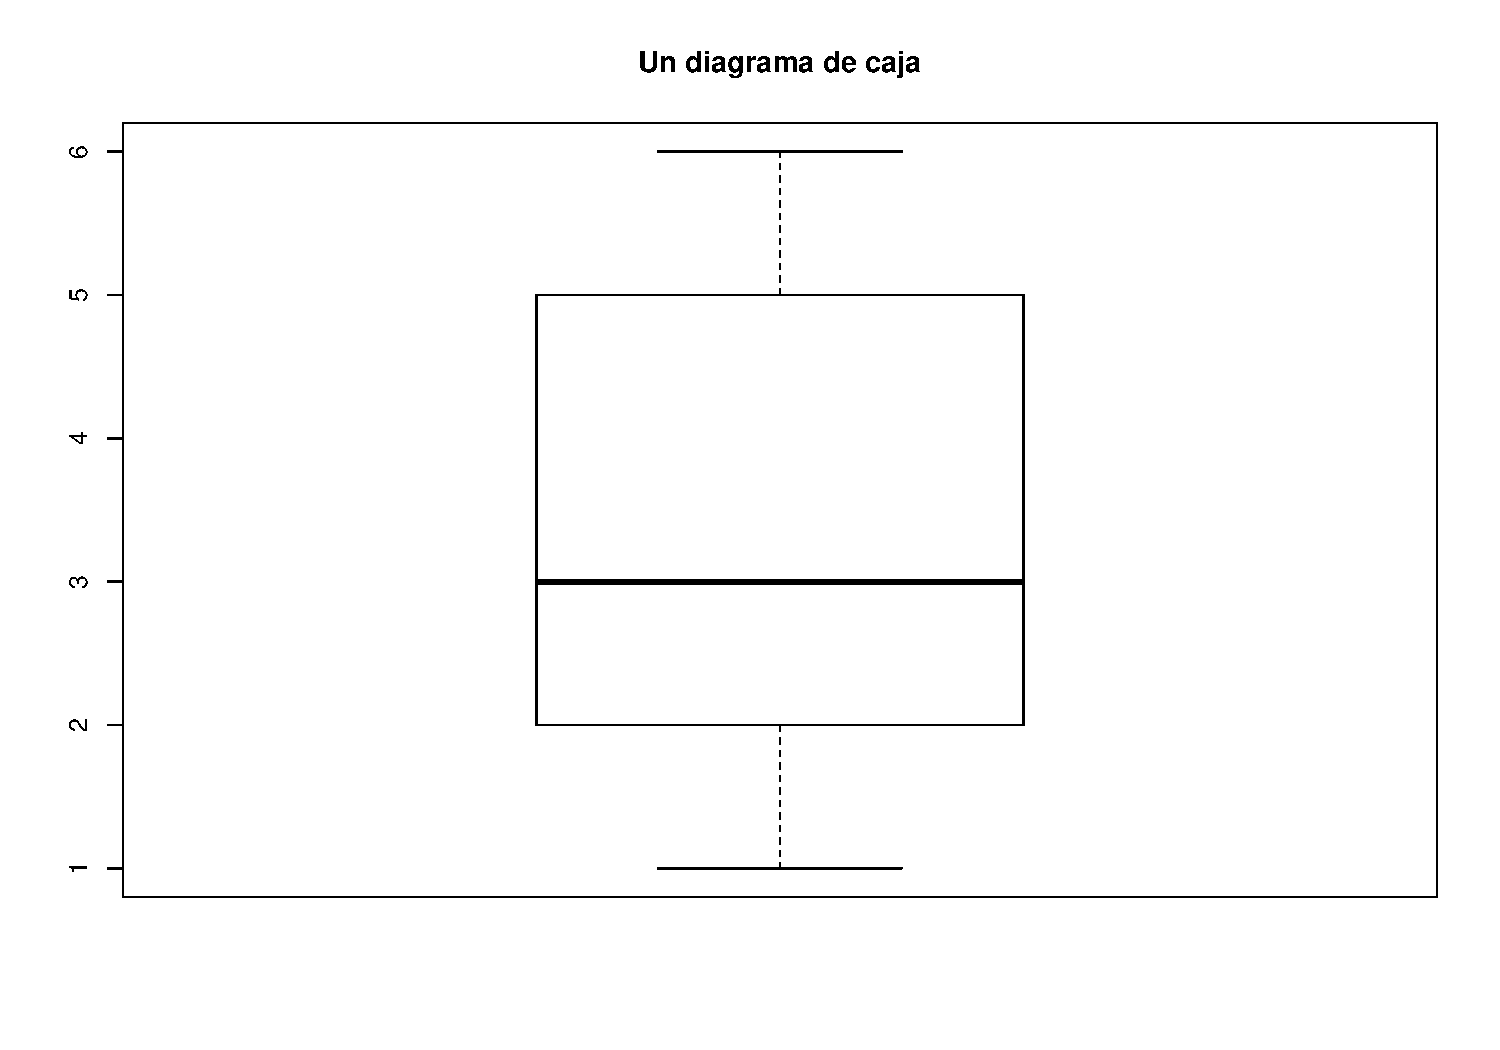
\includegraphics{Tema8.-Datos-Cuantitativos_files/figure-beamer/unnamed-chunk-25-1.pdf}

\end{frame}

\begin{frame}[fragile]{La función boxplot}
\protect\hypertarget{la-funciuxf3n-boxplot-1}{}

También podemos dibujar diversos diagramas de caja en un mismo gráfico.
De este modo, se pueden comparar con mayor facilidad:

\begin{Shaded}
\begin{Highlighting}[]
\KeywordTok{boxplot}\NormalTok{(dado,dados,dados2)}
\end{Highlighting}
\end{Shaded}

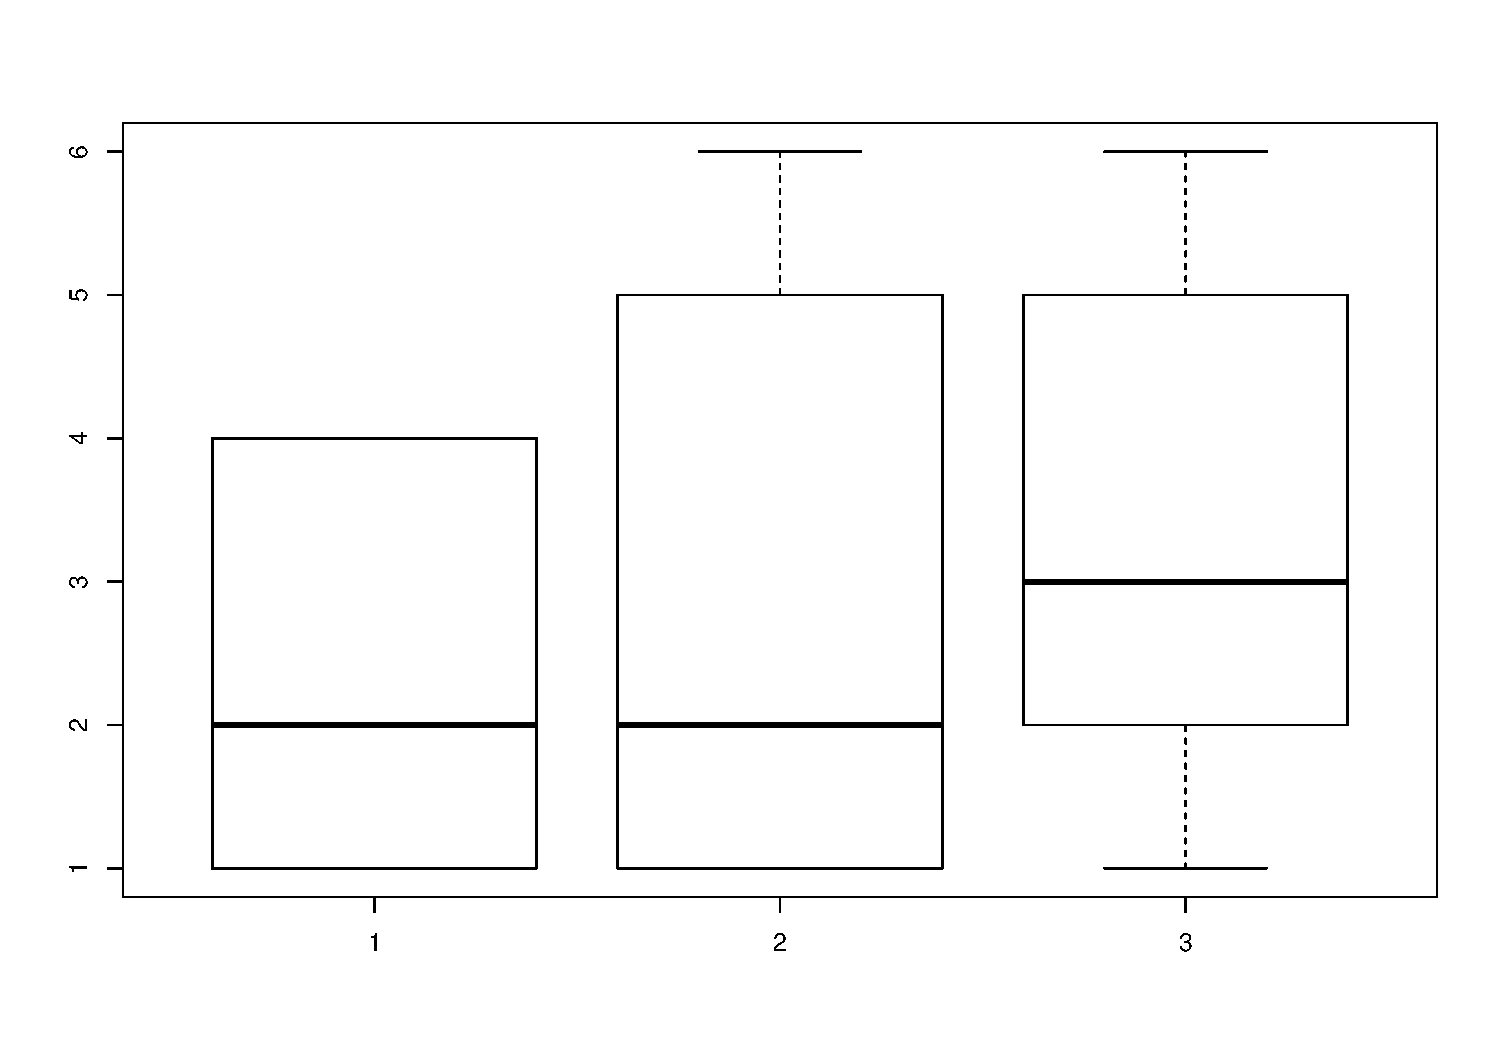
\includegraphics{Tema8.-Datos-Cuantitativos_files/figure-beamer/unnamed-chunk-26-1.pdf}

\end{frame}

\begin{frame}[fragile]{La función boxplot}
\protect\hypertarget{la-funciuxf3n-boxplot-2}{}

Además, podemos dibujar el diagrama de caja de todas las variables de un
data frame en un solo paso aplicando la instrucción
\texttt{boxplot(data.frame)}.

La mayoría de veces, dicho gráfico no será del todo satisfactorio.
Dibujar diagramas de factores no tiene sentido alguno. Estos gráficos se
pueden manipular incluyendo solo las variables de interés, cambiando los
nombres\ldots{}

Veamos un ejemplo:

\end{frame}

\begin{frame}[fragile]{Ejemplo 8}
\protect\hypertarget{ejemplo-8}{}

\begin{Shaded}
\begin{Highlighting}[]
\NormalTok{body =}\StringTok{ }\KeywordTok{read.table}\NormalTok{(}\StringTok{"../data/bodyfat.txt"}\NormalTok{, }\DataTypeTok{header =} \OtherTok{TRUE}\NormalTok{)}
\KeywordTok{boxplot}\NormalTok{(body)}
\end{Highlighting}
\end{Shaded}

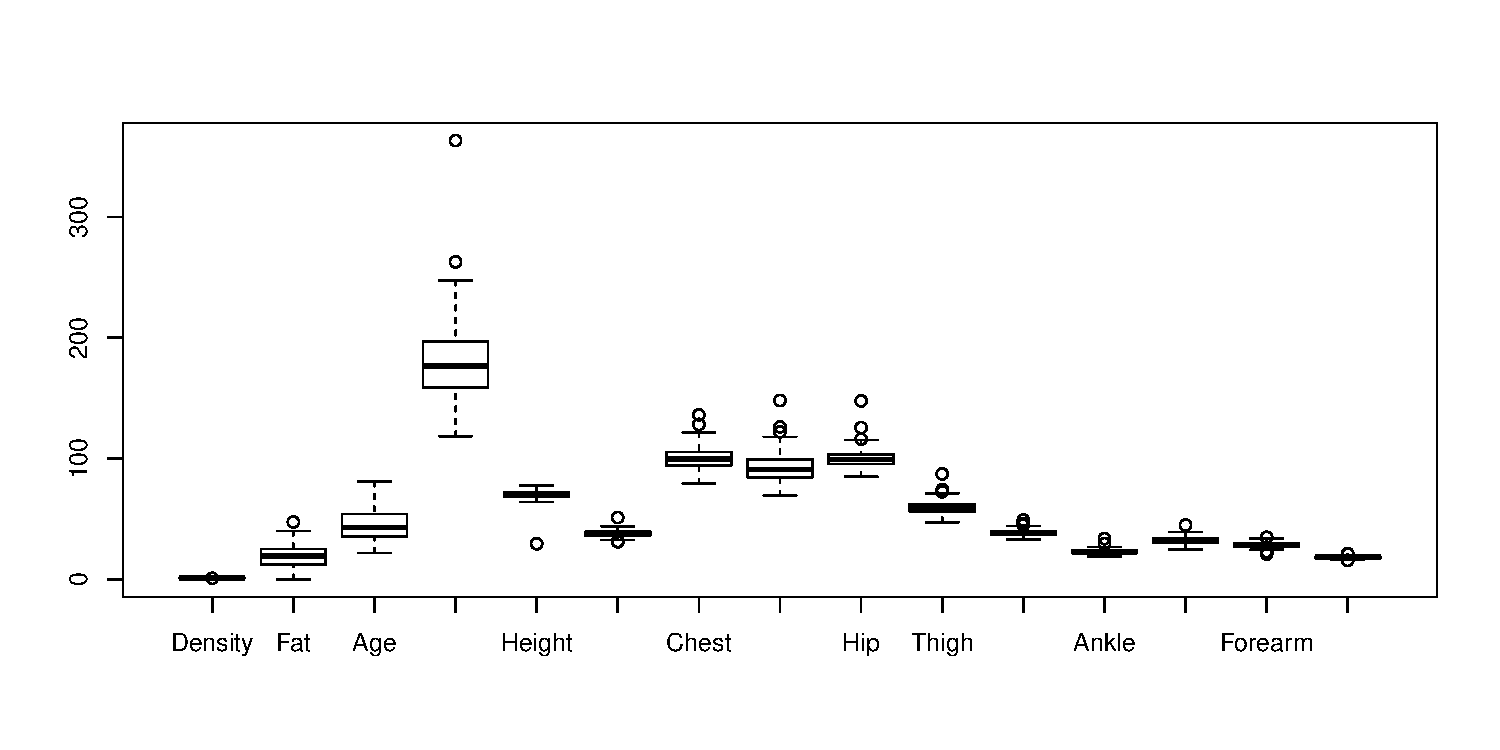
\includegraphics{Tema8.-Datos-Cuantitativos_files/figure-beamer/unnamed-chunk-27-1.pdf}

\end{frame}

\begin{frame}[fragile]{Ejemplo 8}
\protect\hypertarget{ejemplo-8-1}{}

\begin{Shaded}
\begin{Highlighting}[]
\KeywordTok{boxplot}\NormalTok{(body[,}\DecValTok{7}\OperatorTok{:}\DecValTok{9}\NormalTok{], }\DataTypeTok{names =} \KeywordTok{c}\NormalTok{(}\StringTok{"Pecho"}\NormalTok{, }\StringTok{"Abdomen"}\NormalTok{, }\StringTok{"Cadera"}\NormalTok{))}
\end{Highlighting}
\end{Shaded}

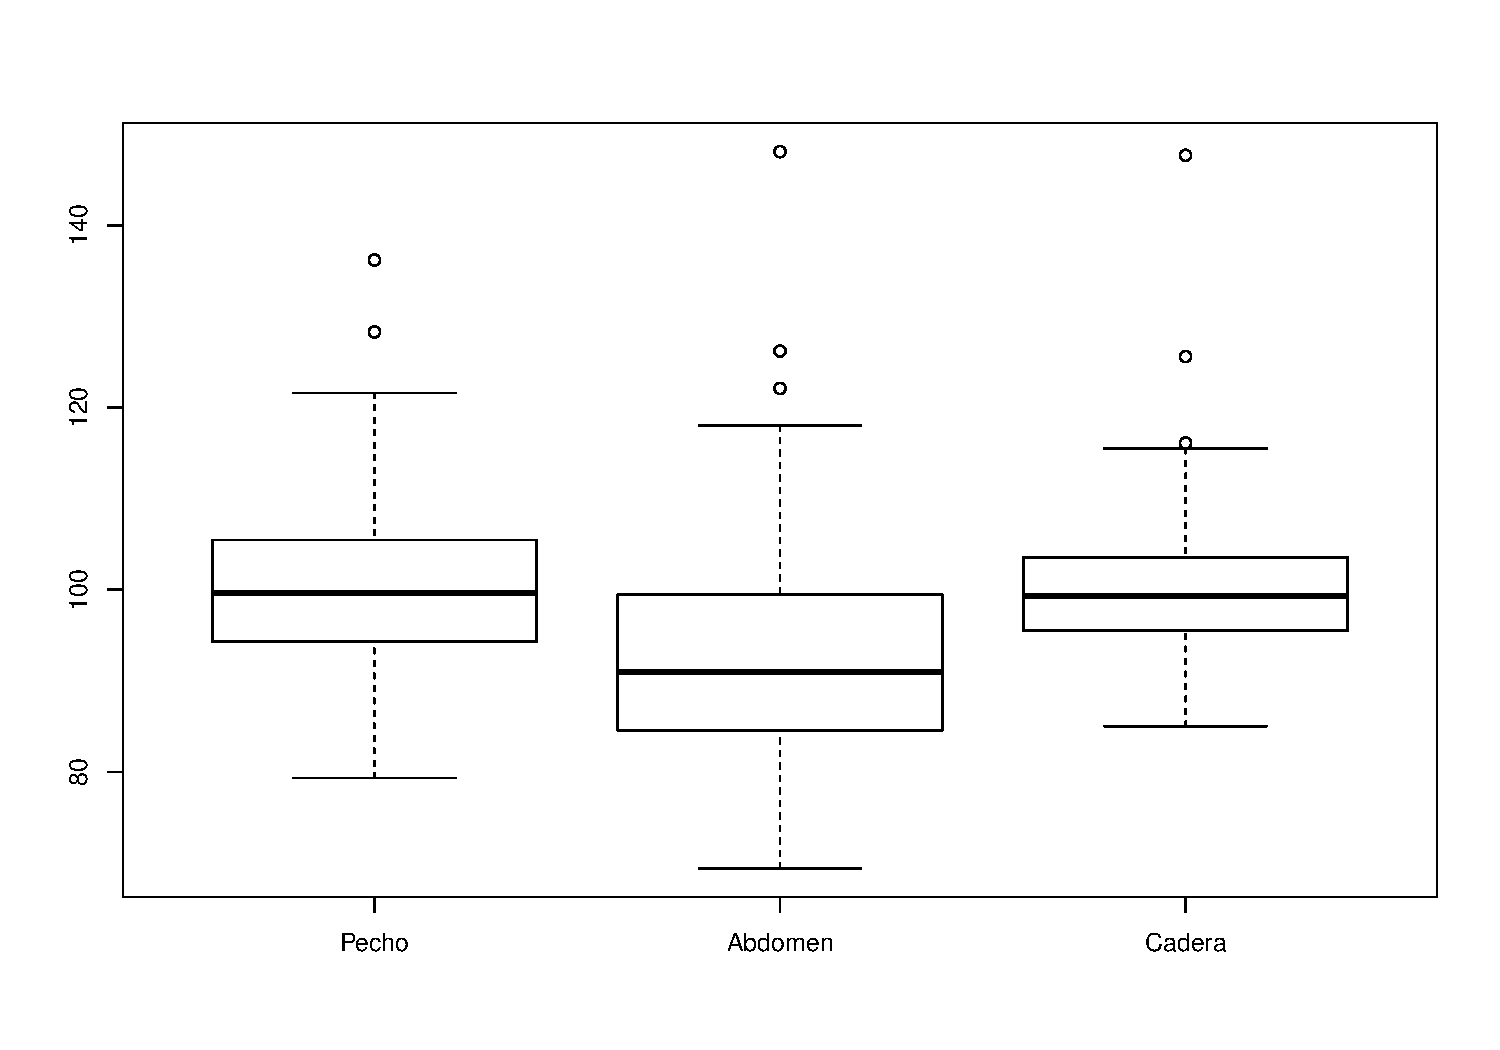
\includegraphics{Tema8.-Datos-Cuantitativos_files/figure-beamer/unnamed-chunk-28-1.pdf}

\end{frame}

\begin{frame}[fragile]{La función boxplot}
\protect\hypertarget{la-funciuxf3n-boxplot-3}{}

Agrupar varios diagramas de caja en un solo gráfico tiene por objetivo
poder compararlos visualmente, lo cual tiene sentido cuando las
variables tienen significados parecidos o cuando comparamos una misma
variable de poblaciones distintas.

La mayoría de las veces, querremos comparar diagramas de cajas de una
misma variable cuantitativa segmentada por los niveles de un factor.

La sintaxis de la instrucción para dibujar en un único gráfico los
diagramas de caja de una variable numérica de un data frame en función
de los niveles de un factor del mismo data frame es
\texttt{boxplot(var.numérica\textasciitilde{}factor,\ data\ =\ data\ frame)}

\end{frame}

\begin{frame}[fragile]{Ejemplo 9}
\protect\hypertarget{ejemplo-9}{}

\begin{Shaded}
\begin{Highlighting}[]
\KeywordTok{boxplot}\NormalTok{(circumference}\OperatorTok{~}\NormalTok{Tree, }\DataTypeTok{data =}\NormalTok{ Orange, }\DataTypeTok{ylab =} \StringTok{"Circunferencia del tronco (mm)"}\NormalTok{, }
        \DataTypeTok{main =} \StringTok{"Boxplot de los naranjos en función del tipo de árbol"}\NormalTok{)}
\end{Highlighting}
\end{Shaded}

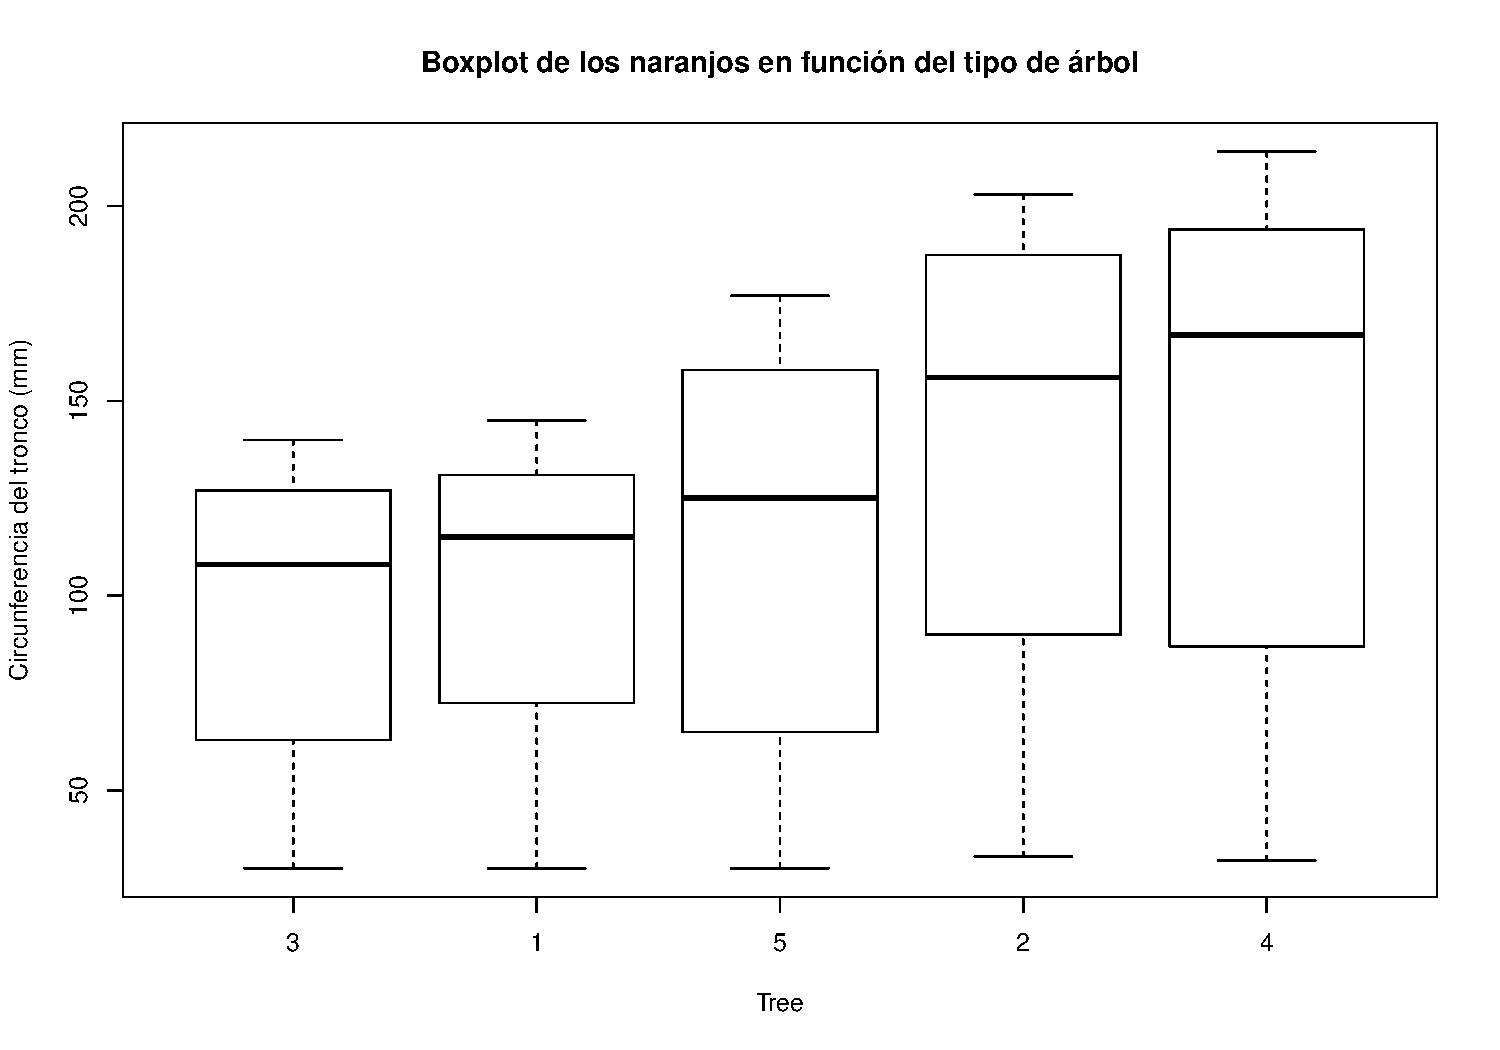
\includegraphics{Tema8.-Datos-Cuantitativos_files/figure-beamer/unnamed-chunk-29-1.pdf}

\end{frame}

\begin{frame}[fragile]{Parámetros de la función boxplot}
\protect\hypertarget{paruxe1metros-de-la-funciuxf3n-boxplot}{}

Todos los parámetros de la función \texttt{plot()} que tengan sentido
pueden ser utilizados en los argumentos de la función
\texttt{boxplot()}.

Aparte, la función \texttt{boxplot()} dispone de algunos parámetros
específicos, de los cuales mencionaremos:

\begin{itemize}
\tightlist
\item
  \texttt{notch} igualado a \texttt{TRUE} añade una muesca en la mediana
  de la caja. Si se da el caso en que las muescas de dos diagramas de
  cajas no se solapan, entonces con alto grado de confianza, concluimos
  que las medianas de las poblaciones correspondientes son diferentes.
\end{itemize}

\end{frame}

\begin{frame}[fragile]{Ejemplo 10}
\protect\hypertarget{ejemplo-10}{}

\begin{Shaded}
\begin{Highlighting}[]
\KeywordTok{boxplot}\NormalTok{(Sepal.Width}\OperatorTok{~}\NormalTok{Species, }\DataTypeTok{data =}\NormalTok{ iris, }\DataTypeTok{ylab =} \StringTok{"Anchura del sétalo (cm)"}\NormalTok{,}
        \DataTypeTok{notch =} \OtherTok{TRUE}\NormalTok{, }\DataTypeTok{col =} \KeywordTok{c}\NormalTok{(}\StringTok{"cyan"}\NormalTok{,}\StringTok{"cyan2"}\NormalTok{,}\StringTok{"cyan4"}\NormalTok{),}
        \DataTypeTok{main =} \StringTok{"Boxplot de iris"}\NormalTok{)}
\end{Highlighting}
\end{Shaded}

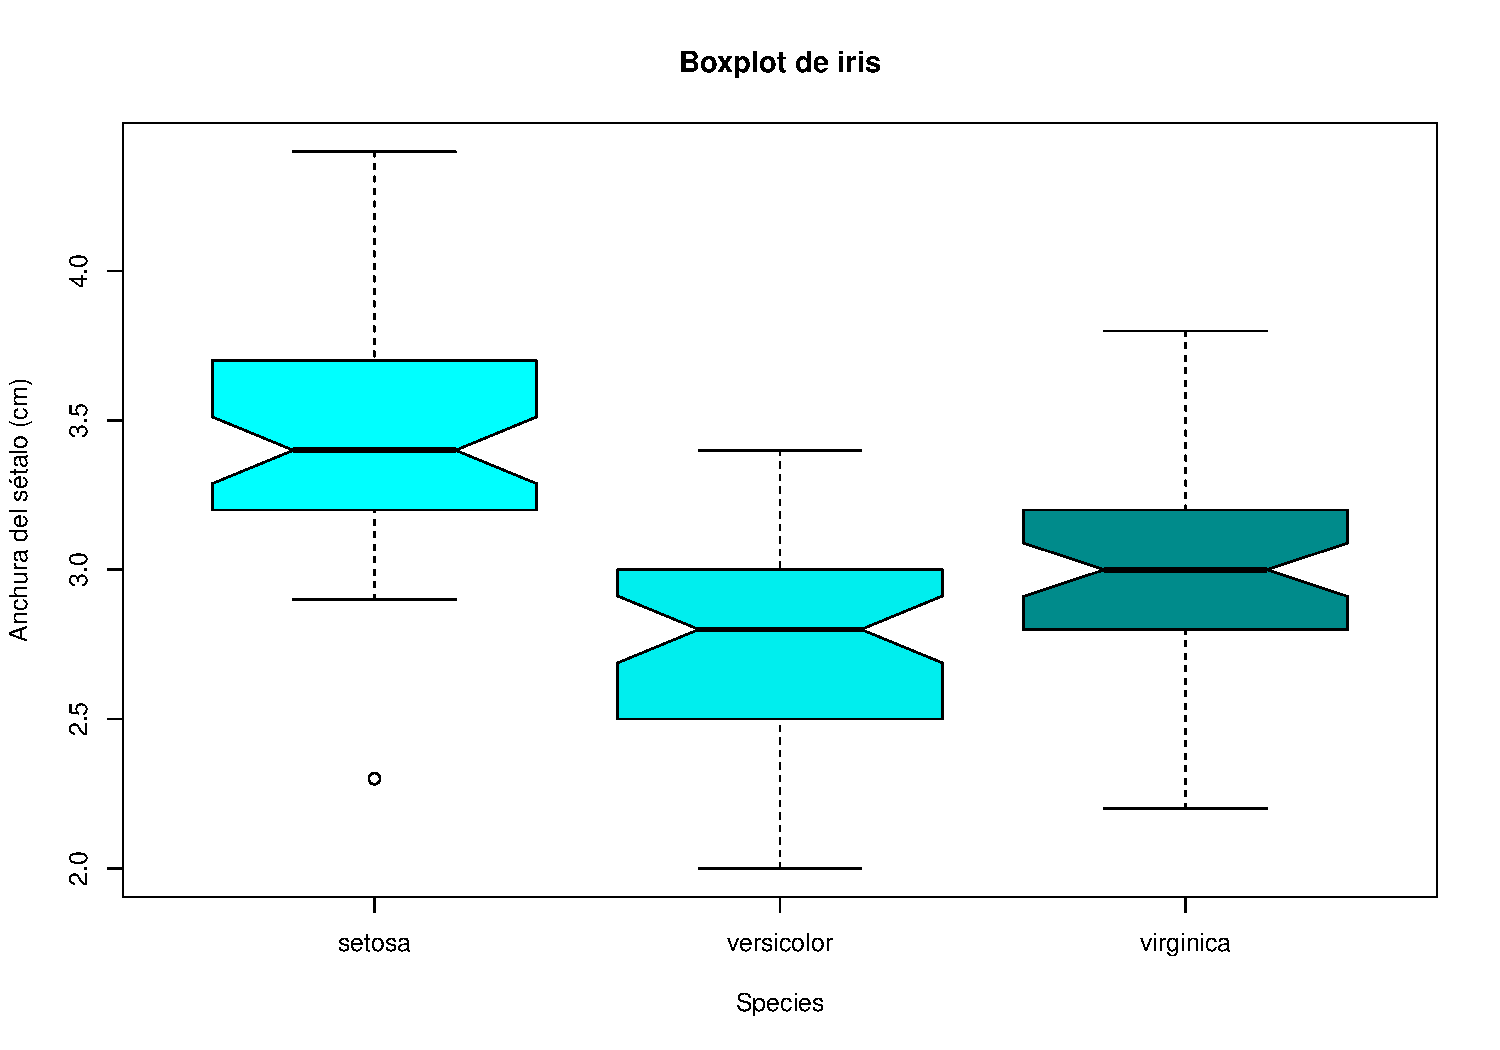
\includegraphics{Tema8.-Datos-Cuantitativos_files/figure-beamer/unnamed-chunk-30-1.pdf}

\end{frame}

\begin{frame}[fragile]{Ejemplo 10}
\protect\hypertarget{ejemplo-10-1}{}

Si quisiéramos marcar de alguna forma en un diagrama de caja, cosa que
puede ser muy útil en ocasiones, la media aritmética de la variable
correspondiente, podríamos hacerlo mediante la función \texttt{points}:

\begin{Shaded}
\begin{Highlighting}[]
\KeywordTok{boxplot}\NormalTok{(Sepal.Width}\OperatorTok{~}\NormalTok{Species, }\DataTypeTok{data =}\NormalTok{ iris, }\DataTypeTok{ylab =} \StringTok{"Anchura del sétalo (cm)"}\NormalTok{)}
\NormalTok{medias =}\StringTok{ }\KeywordTok{aggregate}\NormalTok{(Sepal.Width}\OperatorTok{~}\NormalTok{Species, }\DataTypeTok{data =}\NormalTok{ iris, }\DataTypeTok{FUN =}\NormalTok{ mean)}
\KeywordTok{points}\NormalTok{(medias, }\DataTypeTok{col =} \StringTok{"pink"}\NormalTok{, }\DataTypeTok{pch =} \DecValTok{15}\NormalTok{)}
\end{Highlighting}
\end{Shaded}

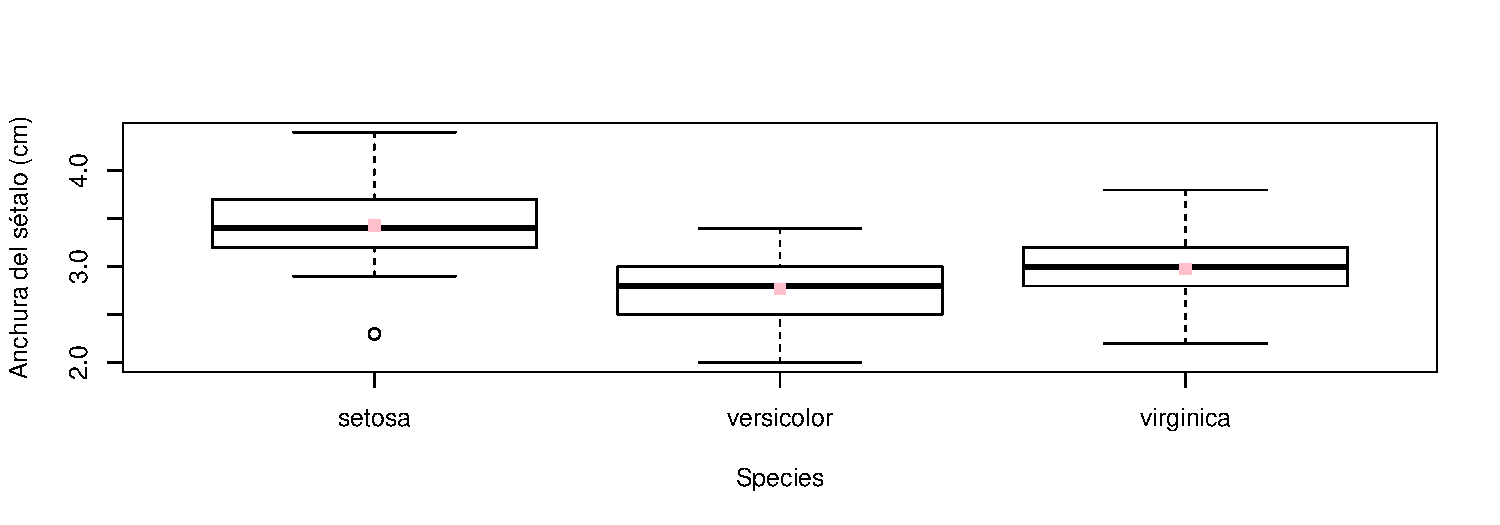
\includegraphics{Tema8.-Datos-Cuantitativos_files/figure-beamer/unnamed-chunk-31-1.pdf}

\end{frame}

\begin{frame}{Ejemplo 10}
\protect\hypertarget{ejemplo-10-2}{}

La primera instrucción del chunk anterior genera el diagrama de cajas de
las anchuras de los sépalos en función de la especie. Por su parte, la
segunda instrucción lo que hace es calcular las medias aritméticas de
las anchuras según la especie. Finalmente, la tercera instrucción lo que
hace es añadir al diagrama un punto cuadrado a cada caja en la ordenada
correspondiente a su media aritmética.

\end{frame}

\begin{frame}[fragile]{La estructura interna de boxplot}
\protect\hypertarget{la-estructura-interna-de-boxplot}{}

Como ya sabemos, podemos estudiar la función interna de algunos objetos
con la función \texttt{str}.

Dicha función aplicada a un boxplot, nos produce una list. Podéis ver
esta list si introducís por consola la siguiente instrucción:
\texttt{str(boxplot(circumference\textasciitilde{}Tree,\ data\ =\ Orange))}
Destacaremos dos de sus componenetes aquí:

\begin{itemize}
\tightlist
\item
  \texttt{stats} nos devuelve los valores
  \(b_{inf},\ Q_{0.25},\ Q_{0.5},\ Q_{0.75},\ b_{sup}\)
\item
  \texttt{out} nos retorna los valores atípicos. En caso de haber
  diversos diagramas en un plot, la componente \texttt{group} nos indica
  a qué diagramas pertenecen estos ouliers.
\end{itemize}

\end{frame}

\end{document}
